%% Standalone supplementary material for the FEBio ringAddedMass comparison.
%% Build (from this directory; article.aux is read for main-article cross-references):
%%   latexmk -pdf article.tex && latexmk -pdf supplement_febio_ring.tex
%% The main article refers to this file as "Supplementary Material, Sec. S1, Figs. S1-S2"
%% when \supplementseparatetrue is set in article.tex (default: Appendix B in article.tex).
\documentclass[sn-mathphys,Numbered]{sn-jnl}
\usepackage{graphicx}
\usepackage{amsmath,amssymb,amsfonts,bm}
\usepackage{xcolor}
\usepackage{manyfoot}
\usepackage{booktabs}
\usepackage{siunitx}
\usepackage{float}
\usepackage[utf8]{inputenc}
\usepackage[onehalfspacing]{setspace}
\usepackage[section]{placeins}
\usepackage{geometry}
\geometry{a4paper,textwidth=15cm,textheight=24cm}
\setlength{\parskip}{\baselineskip}

%% S-prefixed numbering
\renewcommand{\thesection}{S\arabic{section}}
\renewcommand{\thefigure}{S\arabic{figure}}
\renewcommand{\thetable}{S\arabic{table}}
\renewcommand{\theequation}{S\arabic{equation}}

%% Cross-references to the main article (labels prefixed M-)
\usepackage{xr-hyper}
\externaldocument[M-]{article}

\begin{document}

\title[Supplementary material: FEBio comparison for ringAddedMass]{Supplementary material: independent FEBio comparison for ringAddedMass}

\author*[1]{\fnm{Philip} \sur{Cardiff}}\email{philip.cardiff@ucd.ie}
\author[1,2]{\fnm{Ivan} \sur{Batisti\'{c}}}
\author[1]{\fnm{Sairam} \sur{Pamulaparthi Venkata}}

\affil[1]{\orgdiv{School of Mechanical and Materials Engineering}, \orgname{University College Dublin}, \orgaddress{\country{Ireland}}}
\affil[2]{\orgdiv{Faculty of Mechanical Engineering and Naval Architecture}, \orgname{University of Zagreb}, \orgaddress{\country{Croatia}}}

\abstract{Supporting detail for the independent FEBio comparison of the ringAddedMass benchmark in the main article, ``Benchmark problems are not benchmark solutions: an open verification suite for continuum fluid--solid interaction with quantified numerical uncertainty''.}

\maketitle

%%%%%%%%%%%%%%%%%%%%%%%%%%%%%%%%%%%%%%%%%%%%%%%%%%%%%%%%%%%%%%%%%%
\section{FEBio comparison for the ring added-mass problem}
\label{app:ring_febio}
%%%%%%%%%%%%%%%%%%%%%%%%%%%%%%%%%%%%%%%%%%%%%%%%%%%%%%%%%%%%%%%%%%
This supplement gives the supporting detail for the independent FEBio comparison of Section~\ref{M-sec:ring} of the main article (Table~\ref{M-tab:ring_febio}, Figure~\ref{M-fig:ring_febio_ratio}).

\emph{Graded-mesh ladder.}
Controlled refinement of the first fluid cell at both walls (all else fixed: $4\delta$, $\delta$, $\delta/4$, $\delta/16$ for the moderate level, with a potential-flow start) moved the ratio error against the finite-viscosity eigenvalue from $-0.13\%$ to $+0.02$, $+0.001$ and $+0.013\%$ and the fitted decay from an amplitude growth ($-0.47$ times the exact rate at $4\delta$) to $0.56$, $1.02$ and $1.03$ times the exact rate, and reduced the net energy creation over four periods from $1.4\%$ of the initial energy at $4\delta$ to $0.31\%$, $0.26\%$ and $-0.23\%$; neither the time step, the tangential resolution nor the initial fluid velocity changed this behaviour.

\begin{figure}[htbp]
	\centering
	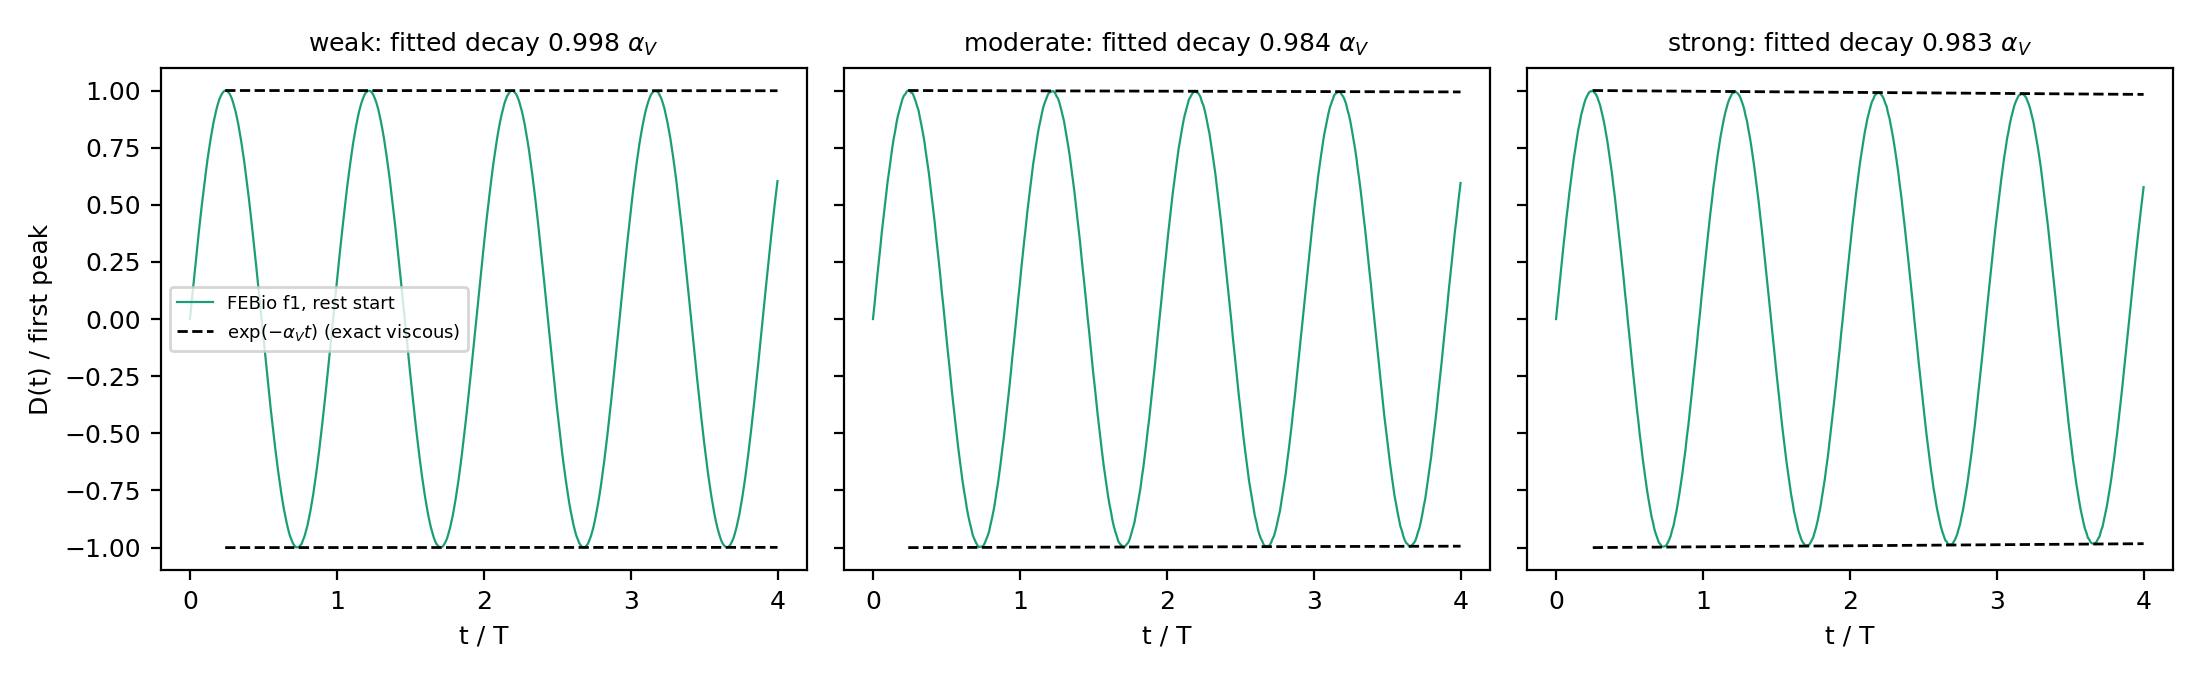
\includegraphics[width=\textwidth]{figures/verification/ringAddedMass_febio_R3}
	\caption{ringAddedMass, FEBio displacement histories $D=(u_r(0^\circ)-u_r(90^\circ))/2$ at the f1 resolution with the fluid at rest, normalised by the first peak, for the weak, moderate and strong levels, with the exact viscous envelope $\exp(-\alpha_V t)$. The fitted decay rates are $0.998$, $0.984$ and $0.983$ times $\alpha_V$.}
	\label{fig:ring_febio_decay}
\end{figure}

\emph{Interface mechanics.}
The pressure and viscous traction that FEBio's fluid--FSI surface load applies to the ring were reconstructed from logged nodal dilatation and element stress (Figure~\ref{fig:ring_febio_traction}).
The work of the reconstructed traction equals the ring's kinetic plus strain energy change to $0.02$--$0.09\%$ of the energy swing ($1.9\%$ for the strong level started at rest), which checks the orientation, the area measure and the sign independently of the force magnitude, and the $n=2$ viscous shear amplitude is $0.84$--$0.90$ of the thin-Stokes-layer estimate computed from the logged velocities, with a shear-to-pressure traction ratio of $4\times10^{-4}$ to $8\times10^{-4}$.
For the strong level started from the potential-flow field, the energy lost by the fluid including the integrated viscous dissipation balances the work on the ring to $0.5\%$ of the ring's energy swing, and the discrete energy balance is closed to $0.3\%$ of the initial energy.
These are reconstructions and one-element-gradient dissipation estimates, not measured interface forces; the weak level started from the potential-flow field did not converge in its first step and is not reported.
\begin{figure}[htbp]
	\centering
	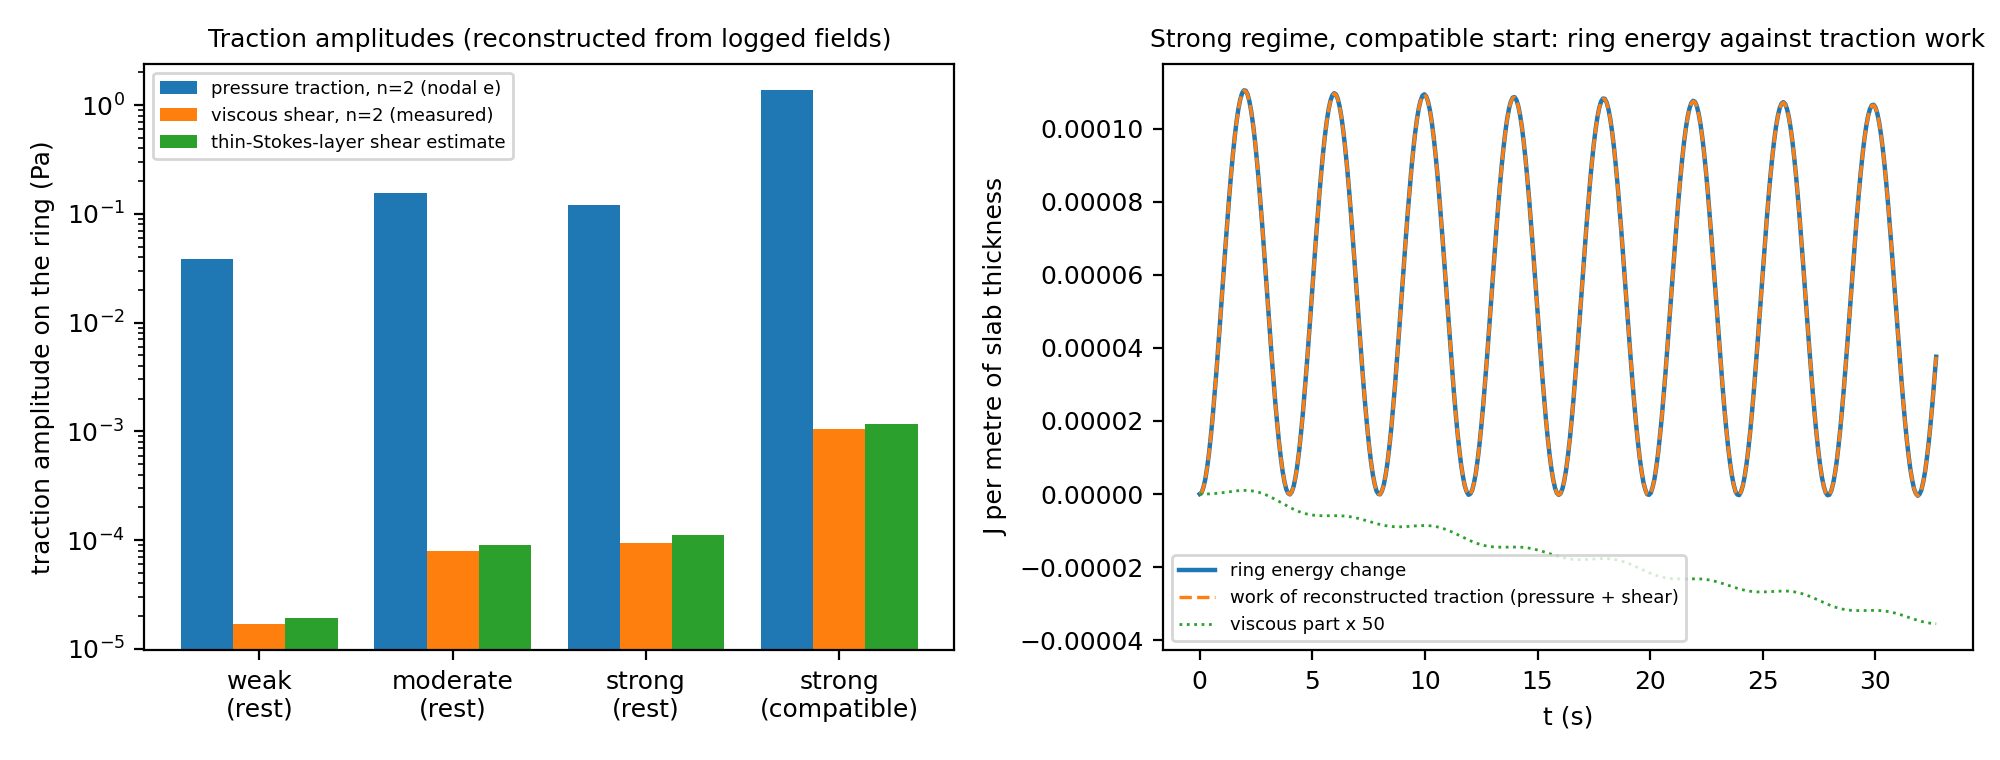
\includegraphics[width=\textwidth]{figures/verification/ringAddedMass_febio_R4}
	\caption{ringAddedMass, FEBio interface traction on the ring, reconstructed from logged fields. Left: $n=2$ amplitudes of the pressure traction, the viscous shear traction and the thin-Stokes-layer shear estimate (fluid at rest, and the strong level from the potential-flow field). Right: strong level, potential-flow start, the ring's energy change and the work of the reconstructed traction (the viscous part, multiplied by 50, is dissipative). Source: \texttt{paper-data/febio\_ring\_added\_mass/no\_slip\_resolved/}.}
	\label{fig:ring_febio_traction}
\end{figure}




\end{document}
